\section{Methodology}
I propose \name, a starting point for an accessible CAPTCHA system, such that the user selects what they can do and are then subjected to a corresponding test.
The system is accessible through a browser\footnote{It is per now not on the internet and can be accessed only locally.}, as it would be realistically desired, and currently supports the following tests:

\paragraph{Text recognition}
A classical text recognition as in CAPTCHA and ReCAPTCHA, in which the user reads a warped text and has to input it to the system, see figure \ref{fig:gui:text_recognition}.
Data were collected from \cite{wilhemy2013dataset,gregwar2022captcha} and the system performs a simple text matching.

\paragraph{Image classification}
One of Luis von Ahn's original ideas for CAPTCHA was to show some image to the user and have them describe it, yet humans proved to be very bad at it.
As an example, given an image of a car people would also say something like "tires", "vehicle", "automobile" and so on, all of which are correct.
Taking inspiration from that I set the up a closed-response object classification task as in figure \ref{fig:gui:image_classification}, images are took from the \emph{Natural Images} dataset used in \cite{roy2018deep}

\paragraph{Finger counting}
The two previous tasks are highly dependent on sight and do not add any accessibility to the system, thus we include a behavioral task: the user is shown a number and a rectangle on the screen and is asked to replicate it with their fingers (figure \ref{fig:gui:finger_count}), if they do it correctly for a customizable interval of time then the test is passed.
The \emph{MMPOSE} toolkit~\cite{mmpose} implements hand pose recognition and even though the model has good performances (AUC of 84\% and PCK@0.2 to 81\%) there are still issues with too high or low illumination - a known problem in computer vision.
The way in which we count finger is based on keypoints' position i.e. when a finger's phalanx keypoint is over its respective knuckle we increment our counter by one.
Doing that we assume the user adopts the western way of finger counting, cultural differences make it impossible to have a universal system: in many regions of Asia the thumb acts as a pointer counting on phalanxes (figure \ref{fig:asian-count}), particular to the Korea Peninsula is \emph{chisanbop} which allows to count up to 99 based on the assignment shown in figure \ref{fig:chisanbop}.
In western countries things are a bit easier to address and each finger is associated to a unit, even though it was not always like that (figure \ref{fig:western-pacioli}), there are still some "regional" variations \ref{fig:inglorious} that the system can take care of.

\begin{figure}[h!t]
    \centering
    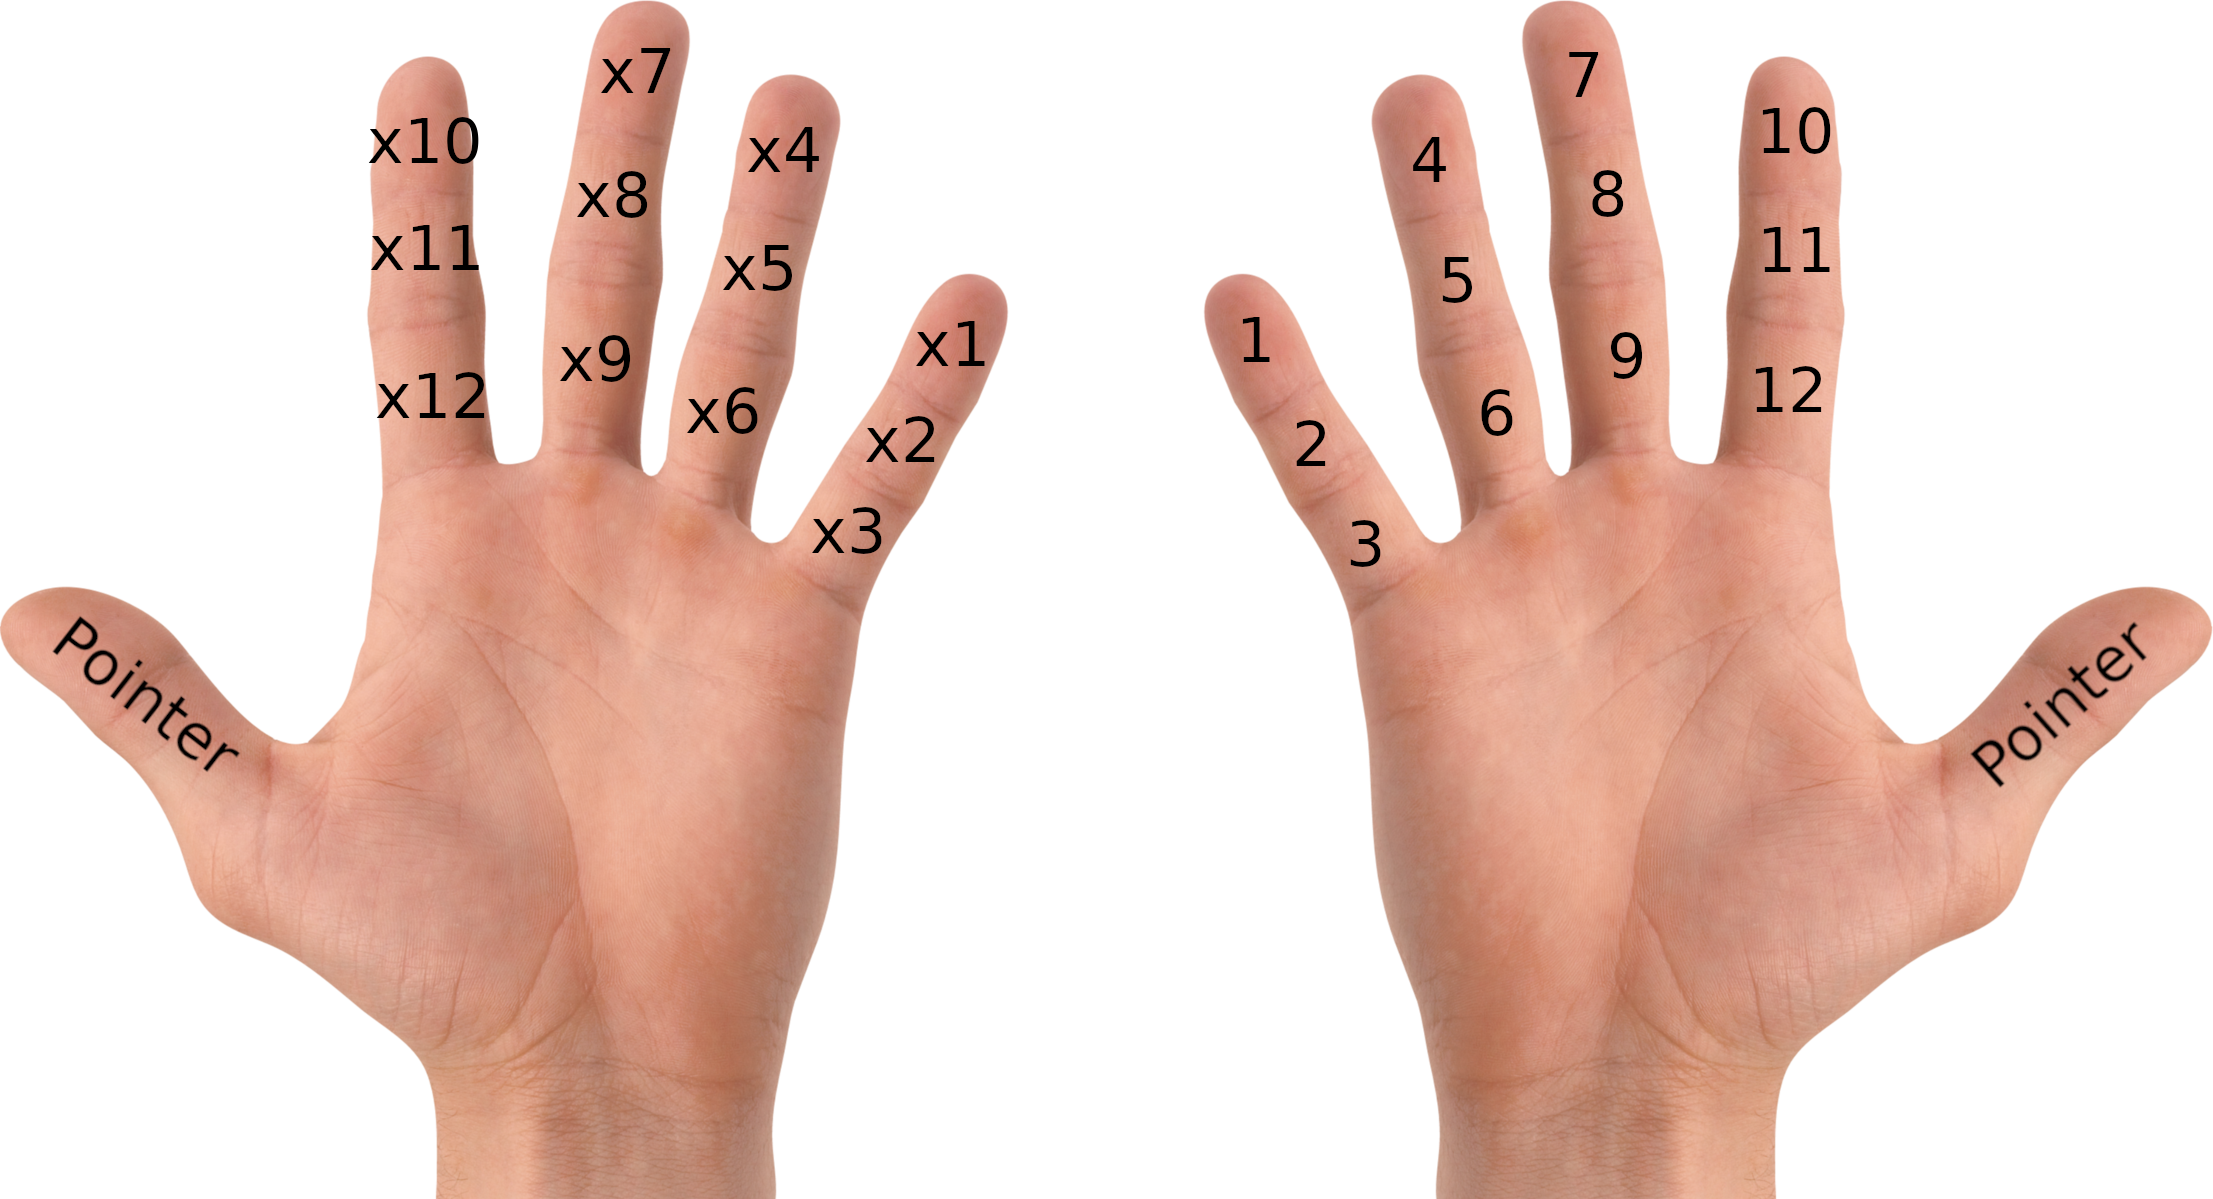
\includegraphics[scale=0.6]{assets/images/finger_count_asia.png}
    \caption{In some regions of Asia finger counting is done on base-12. One hand keeps track of the number and the other acts as a multiplier, up to 144.}
    \label{fig:asian-count}
\end{figure}

\begin{figure}[h!t]
    \centering
    \begin{subfigure}{.49\textwidth}
        \centering
        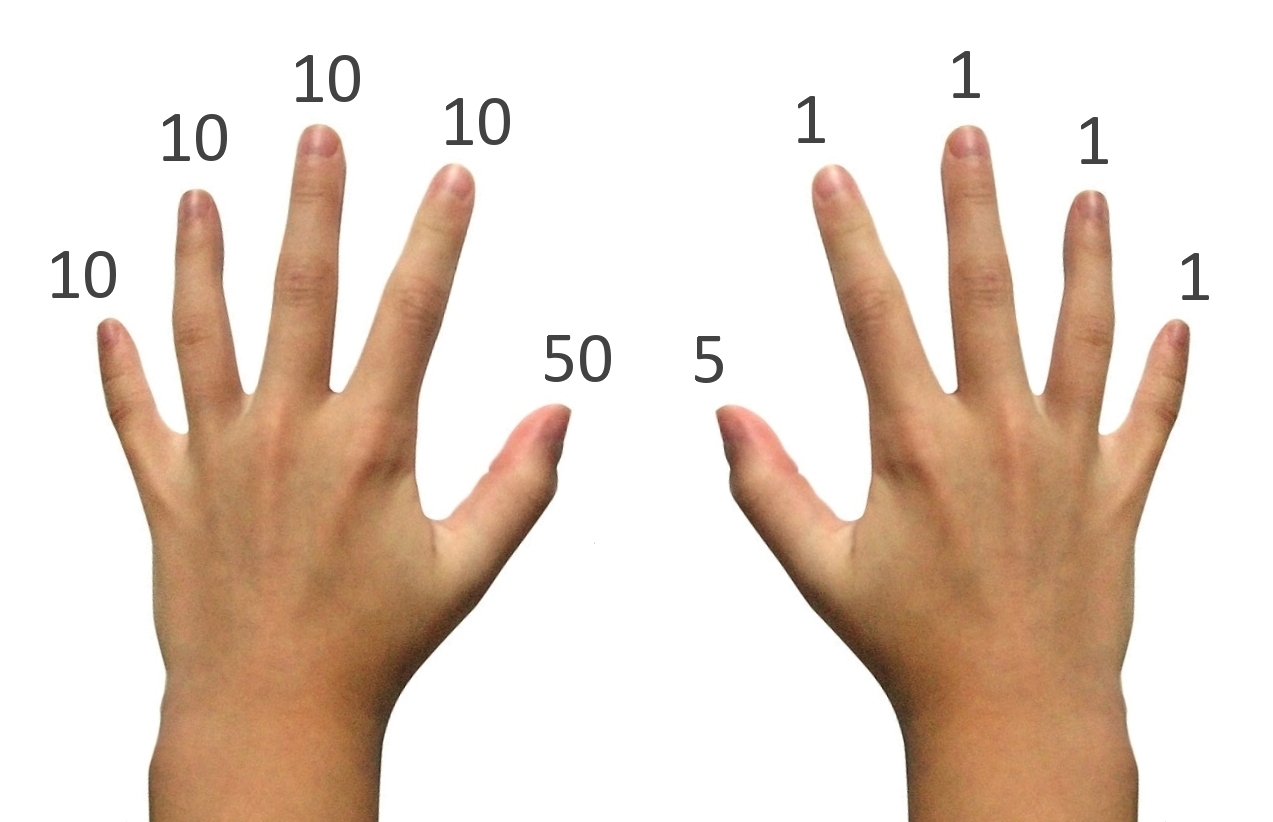
\includegraphics[scale=0.12]{assets/images/chisanbop_numbered.jpg}
        \caption{How to count in chisanbop.}
        \label{fig:chisanbop:system}
    \end{subfigure}
    %
    \begin{subfigure}{.49\textwidth}
        \centering
        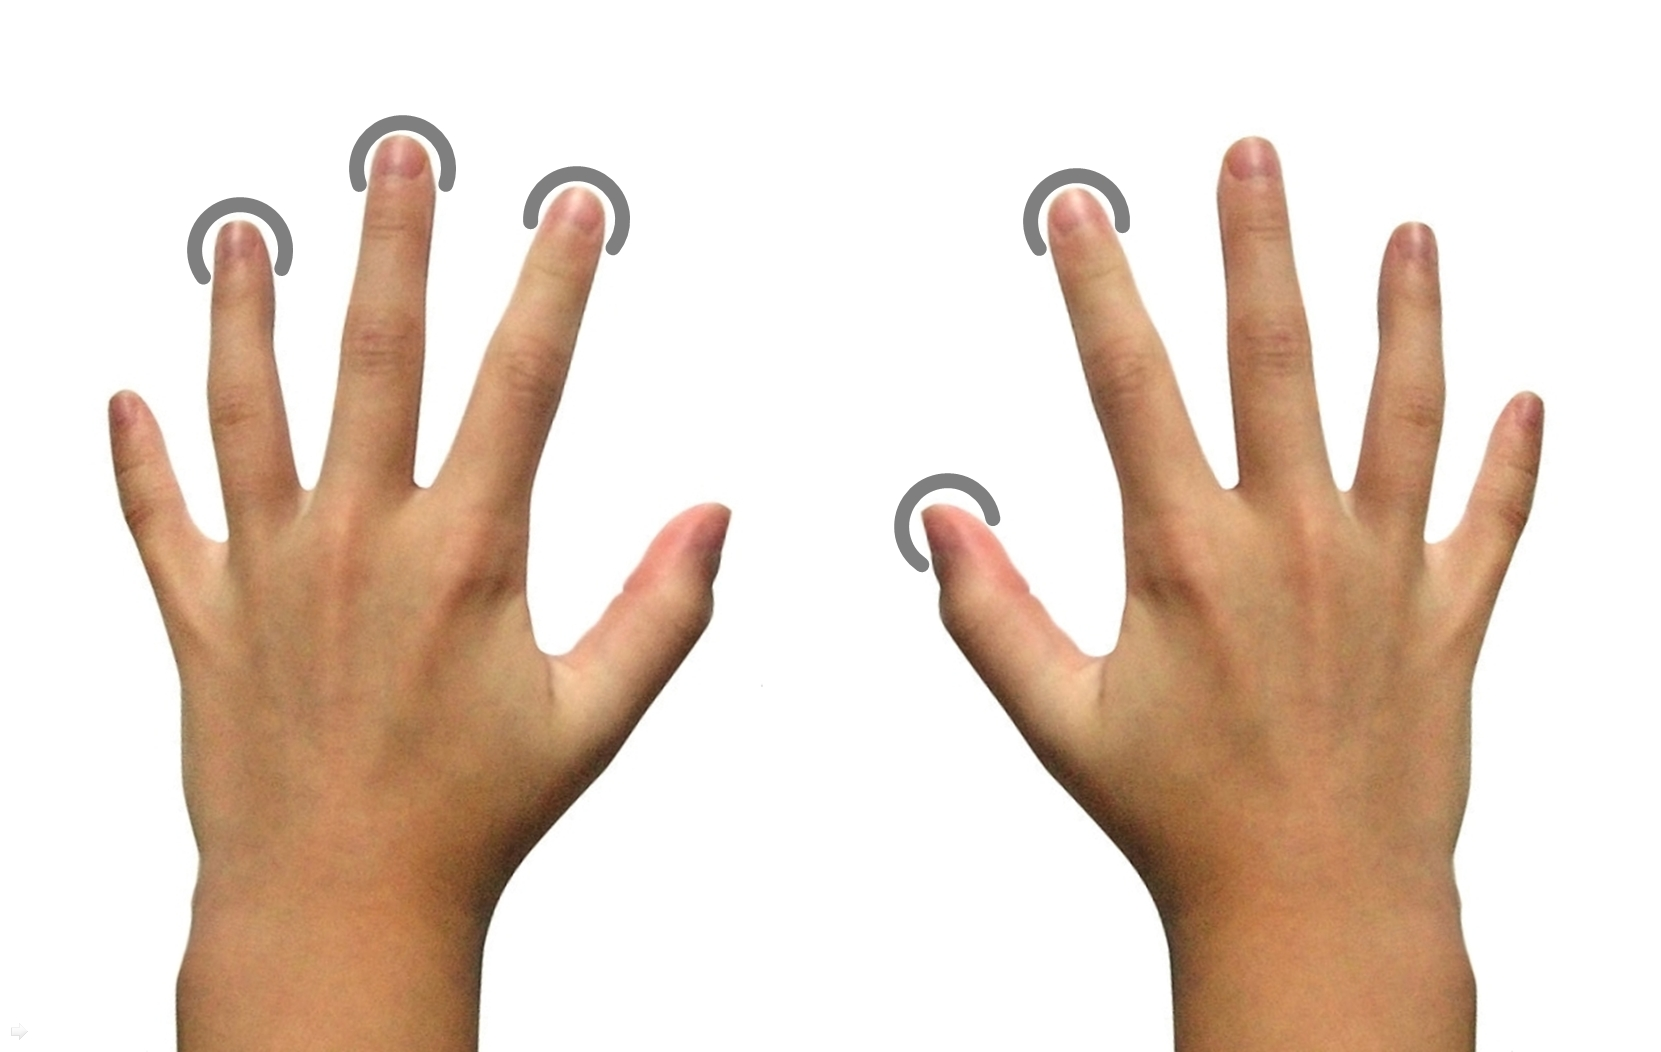
\includegraphics[scale=0.09]{assets/images/chisanbop_36.jpg}
        \caption{Thirty-six in chisanbop.}
        \label{fig:chisanbop:36}
    \end{subfigure}
    \caption{Chisanbop numbering system.}
    \label{fig:chisanbop}
\end{figure}

\begin{figure}[h!t]
    \centering
    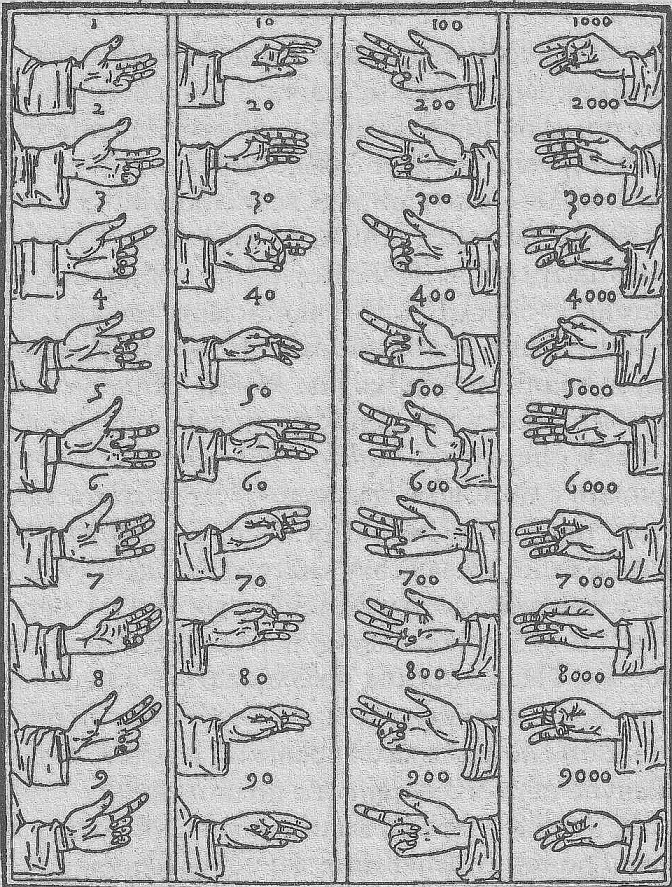
\includegraphics[scale=1]{assets/images/western_pacioli.jpg}
    \caption{Finger numbering system to count from 1 to 9999 from \emph{Summa de arithmetica}, Luca Pacioli, 1494.}
    \label{fig:western-pacioli}
\end{figure}

\begin{figure}[h!t]
    \centering
    \begin{subfigure}{\textwidth}
        \centering
        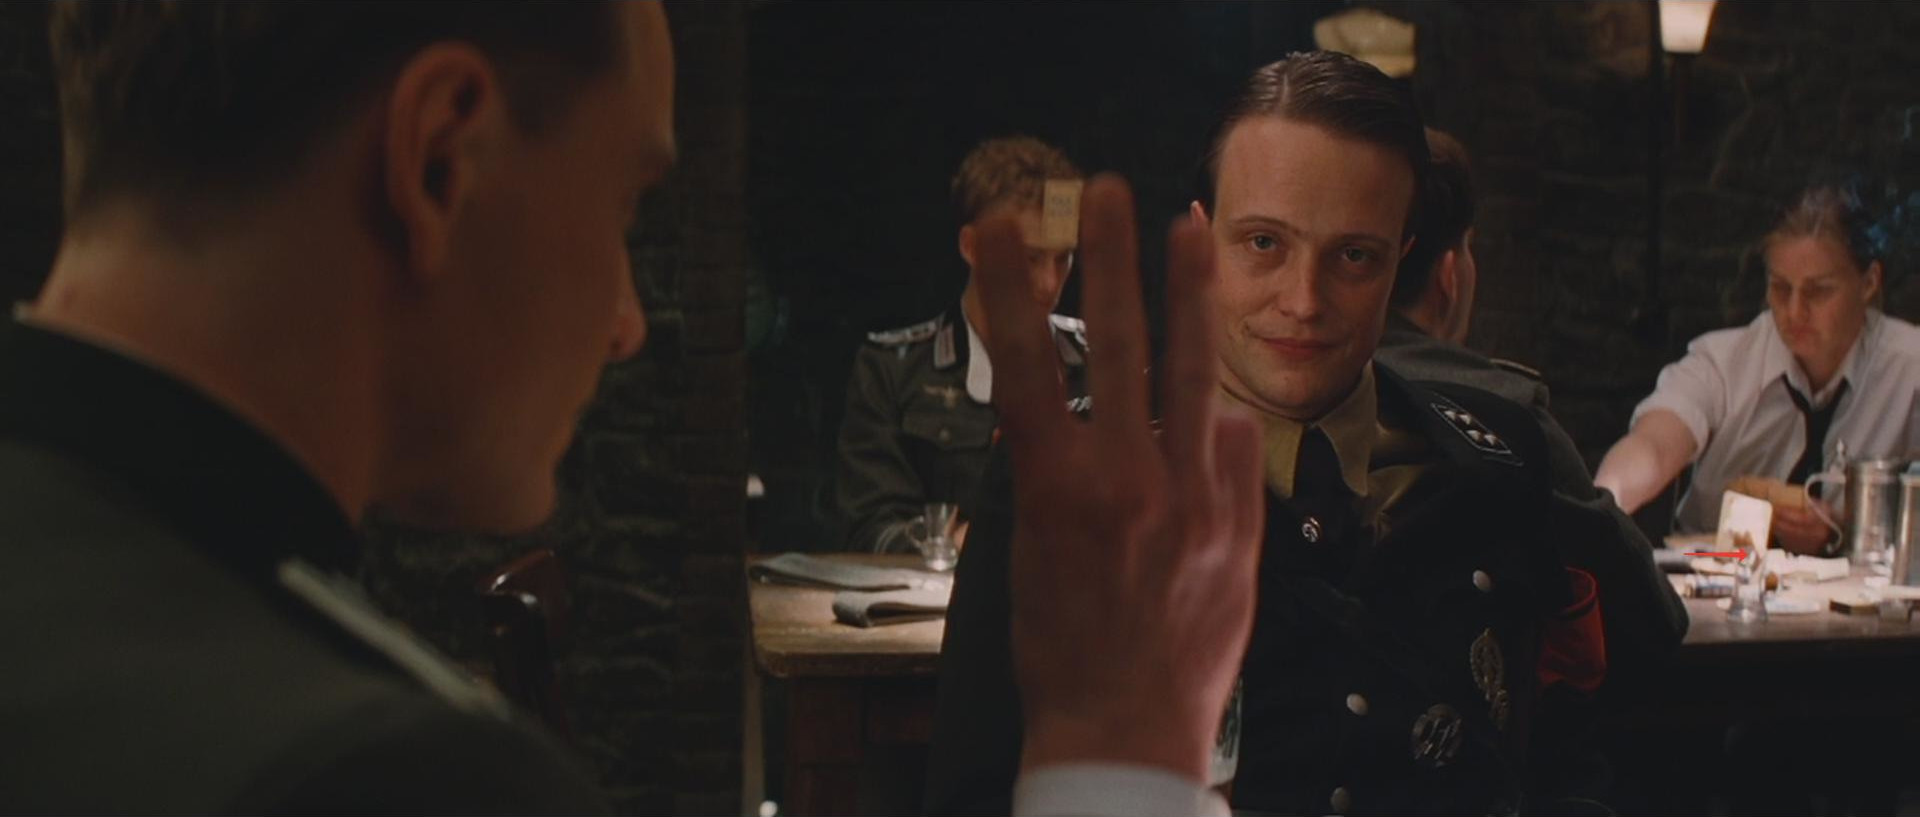
\includegraphics[scale=0.15]{assets/images/inglorious_basterds_english.jpg}
        \caption{Number three as done in Great Britain.}
        \label{fig:inglorious:english}
    \end{subfigure}
    %
    \begin{subfigure}{\textwidth}
        \centering
        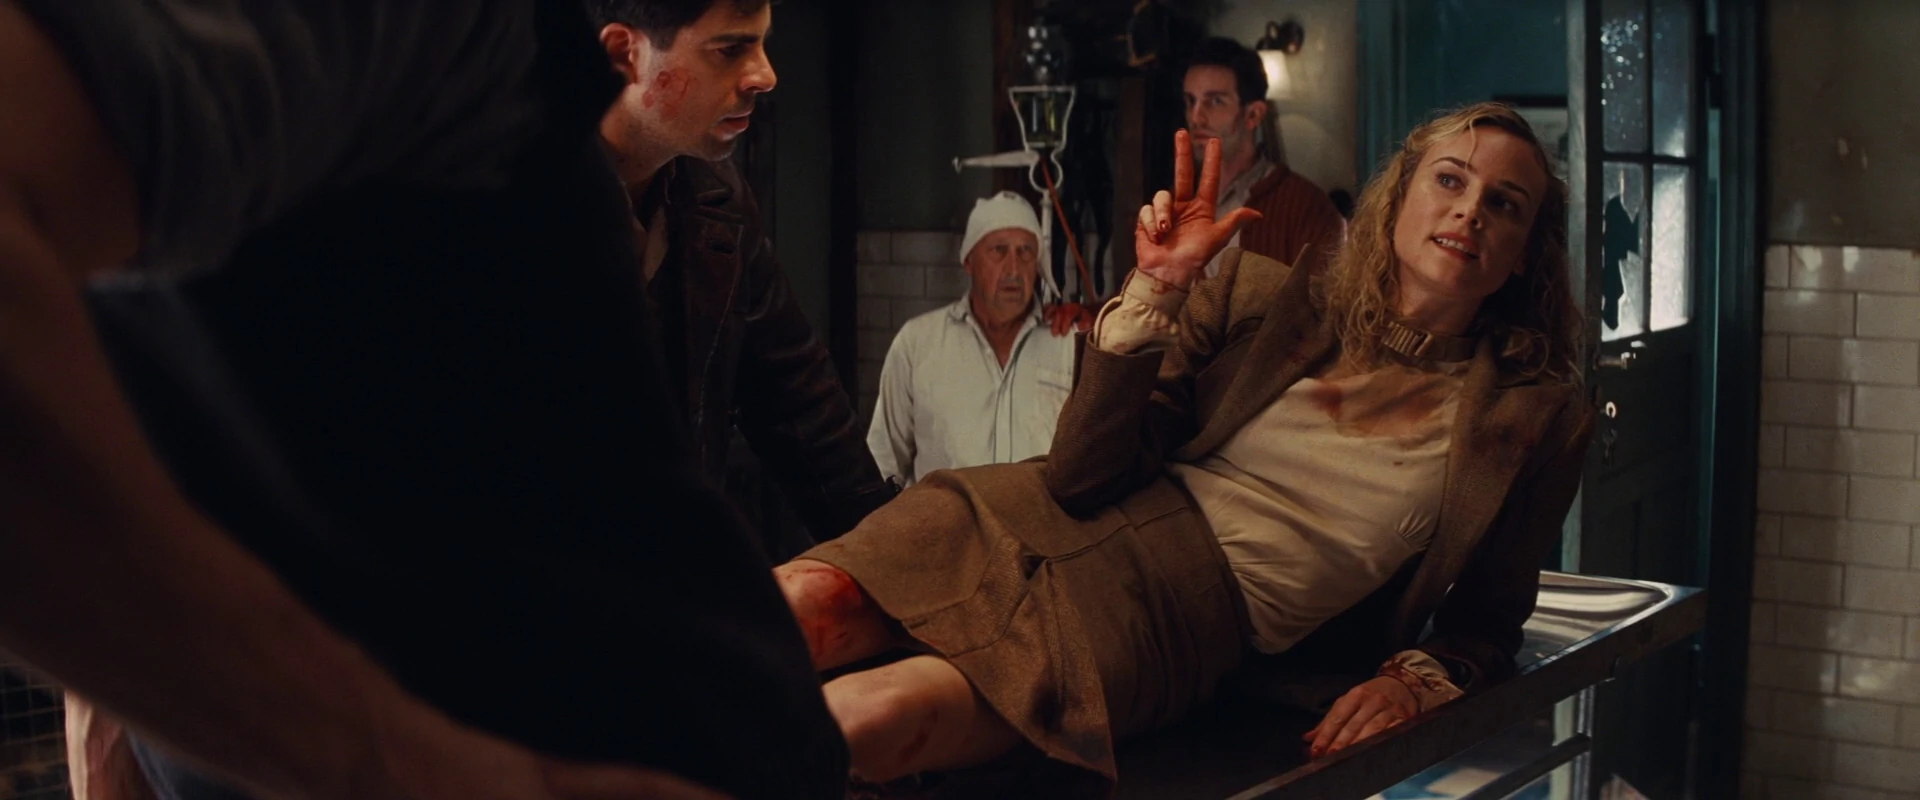
\includegraphics[scale=0.15]{assets/images/inglorious_basterds_german.png}
        \caption{Number three as done in continental Europe.}
        \label{fig:inglorious:german}
    \end{subfigure}
    \caption{Different variations of the number three in Europe, as shown in Quentin Tarantino's \emph{Inglorious Basterds}.}
    \label{fig:inglorious}
\end{figure}


\paragraph{Word reading}
This task makes use of voice, the system randomly selects a customizable number of words from \cite{dwyl2022engwords} and the user reads them, see figure \ref{fig:gui:word_reading}.
The system uses \emph{Google Cloud Speech API}~\cite{google2022speech}, mainly because is the easiest one to use and does not need us to authenticate for an API token.
Yet be wary that it is not suitable for non-private use cases, and it does not perform good when the user has a non-english accent, italian in our case.

When a user accesses the system they have to configure it according to which tests they can or want to be submitted to, as shown in figure \ref{fig:gui:configure}, by default all chechboxes are unchecked.
The way it is done is by associating each test to a propositional logic conjuction of checkbox flags, then one test is randomly selected from the set of tests whose formula is true.
